\section{Experiments}

\begin{figure*}
    \centering
    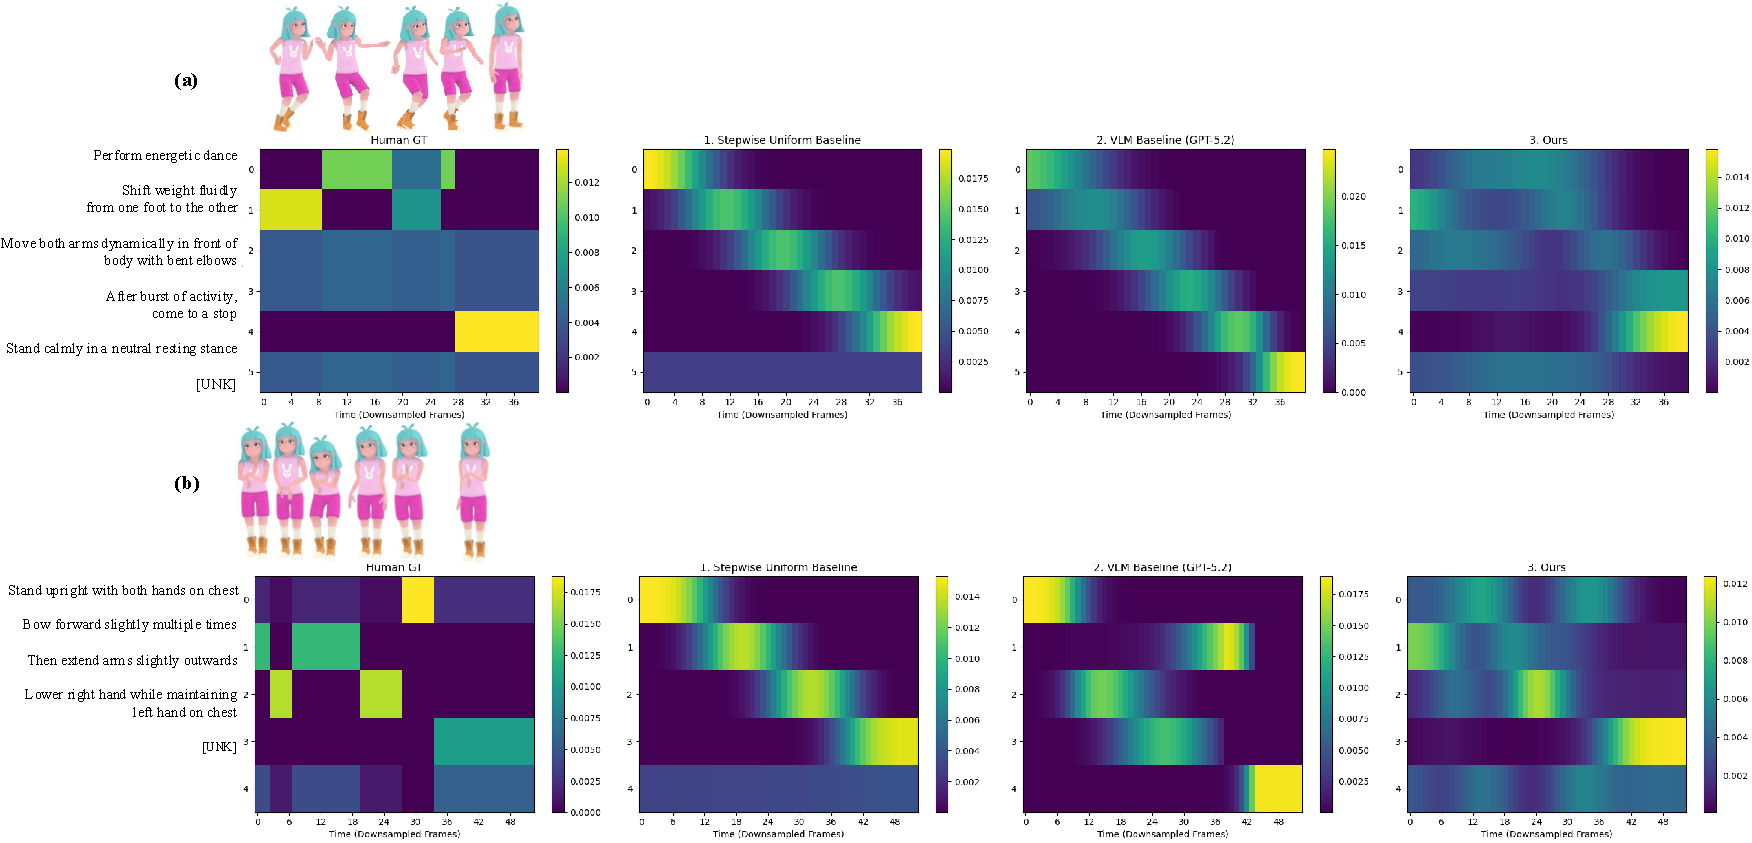
\includegraphics[width=1.05\linewidth]{author-kit-CVPR2026-v1-latex-/figs/qual1.pdf}
    \caption{Qualitative comparison with baselines. We plot the ground truth transport plan and those produced by different methods. Our method produces transport plans that are structurally similar to the ground truth.}
    \label{fig:qual1}
    \vspace{3mm}
\end{figure*}
\subsection{Setting and Implementation Details}
\paragraph{Dataset.} We conduct our experiments on the SnapMoGen dataset~\cite{guo2025snapmogen}, a comprehensive collection of high-fidelity human motion capture data paired with rich textual descriptions. The dataset comprises 34,750 training sequences and 2,012 validation sequences. All motions are originally recorded at 30 FPS. Following SnapMoGen~\cite{guo2025snapmogen}, we downsample the sequences by a factor of 4, resulting in an effective frame rate of 7.5 FPS for both the motion embeddings and the alignment computation. We choose a set of $30$ motion-text pairs from the test set and manually label the ground truth alignment matrix $\mathbf{P}^{gt} \in \mathbb{R}^{T_m \times T_t}$, where $T_m$ and $T_t$ denote the number of downsampled motion frames and atomic action segments, respectively. The details of the labeling process are deferred to the supplementary.

\paragraph{Evaluation Metrics.} \label{paragraph:eval_metric}
We evaluate the alignment accuracy by measuring the discrepancy between the transport matrix $\mathbf{P}$ and the ground-truth annotations $\mathbf{P}^{gt}$. Specifically, we compute the normalized $\ell_1$ distance between the two matrices: 
\begin{equation}    
d(\mathbf{P}, \mathbf{P}^{gt}) = \frac{1}{T_m \times T_t} \sum_{i=1}^{T_m} \sum_{j=1}^{T_t} \left| {\mathbf{P}}_{ij} - {\mathbf{P}}^{gt}_{ij} \right|
\end{equation}

where both matrices are first normalized via the Sinkhorn-Knopp algorithm to enforce doubly stochastic constraints. This ensures they satisfy the predefined row and column marginals (i.e., $\sum_j {\mathbf{P}}_{ij} = 1/T_m$ and $\sum_i {\mathbf{P}}_{ij} = 1/T_t$).

\paragraph{Implementation details.}
Our framework is implemented in PyTorch and trained on a single NVIDIA L40 GPU. Training for 500 epochs takes approximately 12 hours. We use AdamW as the optimizer with an initial learning rate of $2 \times 10^{-4}$ and a batch size of 128. For text encoding, we adopt a frozen T5-base backbone followed by five trainable residual MLP blocks, which project the text features into a 512-dimensional embedding space. For Sinkhorn-based alignment, we set the entropy regularization parameter to $\epsilon=0.1$ and use 50 forward iterations, which we find sufficient for stable convergence in practice. The contrastive temperature is set to $\tau=0.07$. In practice, $T_m$ is typically around 50, while $T_t$ is typically around 5.\\

\subsection{Comparison with Baselines} 
\paragraph{Stepwise Uniform Baseline.} To demonstrate the necessity of dynamic alignment, we construct a stepwise uniform baseline, which inherently assumes a naive, sequential progression between textual actions and motion segments. Specifically, given a motion sequence of $T_m$ frames and $N$ textual actions, this baseline constructs an initial binary matrix by uniformly allocating exactly $\lfloor T_m / N \rfloor$ consecutive frames to each action index in chronological order. Note that the resulting matrix is not strictly block-diagonal; applying the Sinkhorn-Knopp algorithm enforces marginal distribution constraints, which naturally softens the hard boundaries and diffuses the alignment probabilities toward adjacent frames.

\paragraph{VLM Baseline.} To establish a competitive baseline against state-of-the-art vision-language reasoning, we leverage GPT-5.2~\cite{singh2025openai} as a zero-shot temporal segmenter. We give rendered frames sampled at $2.0$ FPS and segmented action-bearing phrases to the VLM and ask it to find the alignment. Details are in the supplementary.

    


    % \item dataset and metrics, including P annotation process: \\

    % Furthermore, we analyze the Argmax Path—defined as the sequence of most probable action-frame assignments—to assess the temporal coherence and the precision of the recovered action boundaries.
    
    % \paragraph{Quantitative Evaluation}
    % We evaluate the alignment performance using the \textbf{Normalized $L_1$ Distance} on the transport plan $P$. To ensure a fair comparison under consistent marginal constraints, both the ground truth (GT) and predicted matrices are normalized using the \textbf{Sinkhorn-Knopp algorithm} such that they satisfy row and column sum constraints (i.e., $\sum_j P_{ij} = 1/T_m$ and $\sum_i P_{ij} = 1/T_t$).

    
    % \paragraph{Results and Analysis}
    % The evaluation reveals several critical insights:
    % \begin{enumerate}
    %     \item \textbf{The ``Semantic Gap'' in LLMs:} Interestingly, as shown in table \ref{tab:alignment_results}, the LLM baseline (\textbf{0.0029}) performs worse than a simple \textbf{Uniform Baseline} (\textbf{0.0027}). This indicates that while GPT-4o possesses strong high-level semantic knowledge, its ``temporal micro-perception'' at the frame level is prone to over-confident misalignments, which are penalized more heavily than a conservative uniform distribution in the Optimal Transport (OT) sense. \\
        % \item \textbf{Superior Micro-Perception:} Our proposed model, even in its \textbf{Raw} form (\textbf{0.0024}), significantly outperforms both the statistical baseline and the LLM. This confirms that our latent-space Sinkhorn Attention learns a more robust mapping between motion dynamics and textual descriptions than explicit visual reasoning on raw frames.
        % \item \textbf{Boundary Precision:} Adopting a ``Nearest-Neighbor'' reassignment and Gaussian smoothing (Post-processed) further refines the alignment to \textbf{0.0022}. This represents a \textbf{25.9\% accuracy gain} over GPT-4o, demonstrating that our model not only understands \textit{what} is happening but precisely \textit{when} the physical transition occurs at a granular level. \\
    % \end{enumerate}  
    

\begin{table*}[t]
\centering
\caption{Quantitative results. Values are reported in normalized $\ell_1$ distance ($\times 10^{-2}$), where lower is better. GF indicates whether to use the global feature. MLP Enc. determines whether to use an MLP-based text encoder or a self-attention-based text encoder.} 
\label{tab:alignment_results}
\begin{tabular}{lcccc}
\toprule
Method & GF & MLP Enc. & temperature & Normalized $\ell_1 \downarrow$ \\
\midrule

Stepwise Uniform Baseline & & & & 0.347 \\
VLM Baseline (GPT-5.2) & & & & 0.296 \\

\midrule
Ours (GF + MLP encoder) & \checkmark & \checkmark & 0.07 & \textbf{0.225} \\
Ours (GF + MLP encoder) & \checkmark & \checkmark& 0.01 & 0.230 \\
Ours (GF + MLP encoder) & \checkmark & \checkmark& 0.03 & 0.237 \\
Ours (GF + attention encoder) & \checkmark  & $\times$ & 0.07 & 0.275 \\
Ours (MLP encoder) & $\times$ & \checkmark & 0.07& 0.239 \\

\bottomrule
\end{tabular}
\end{table*}


% \begin{table*}[t]
% \centering
% \caption{Quantitative results. Values are reported in normalized $\ell_1$ distance ($\times 10^{-2}$), where lower is better. GF indicates whether to use the global feature. MLP Enc. determines whether to use an MLP-based text encoder or a self-attention-based text encoder.} 
% \label{tab:alignment_results_temp}
% \begin{tabular}{lccc}
% \toprule
% Method & GF & MLP Enc. & Normalized $\ell_1 \downarrow$ \\
% \midrule

% Stepwise Uniform Baseline & & & 0.347 \\
% VLM Baseline (GPT-5.2) & & & 0.296 \\

% \midrule
% Ours (GF + MLP encoder, temp = $0.07$) & \checkmark & \checkmark & \textbf{0.225} \\
% Ours (GF + MLP encoder, temp = $0.01$) & \checkmark & \checkmark & 0.230 \\
% Ours (GF + MLP encoder, temp = $0.03$) & \checkmark & \checkmark & 0.237 \\
% Ours (GF + attention encoder) & \checkmark  & $\times$  & 0.275 \\
% Ours (MLP encoder) & $\times$ & \checkmark & 0.239 \\

% \bottomrule
% \end{tabular}
% \end{table*}

\paragraph{Results.} \Cref{tab:alignment_results} presents the quantitative evaluation of our proposed model. The results demonstrate that \ours achieves a significant relative error reduction over the VLM and stepwise uniform baselines. These results demonstrate the necessity of our dedicated data-driven alignment framework.

\subsection{Ablation} 
\paragraph{Impact of the Global Feature Mechanism.} 
A key component of our alignment module is the global feature, which acts as an \texttt{[UNK]} token to absorb transitional or semantically ambiguous frames. In practice, frames near action boundaries often do not correspond strongly to any specific text token. Without such a token, optimal transport tends to force these frames onto neighboring action tokens, leading to blurred boundaries. During evaluation, we reassign the accumulated probability of the \texttt{[UNK]} token strictly to the preceding valid action token. By introducing the global feature, our model can naturally capture these uncertain frames and preserve cleaner temporal segmentation. As shown in \Cref{tab:alignment_results}, this design consistently improves alignment performance over the variant without a global token.

\paragraph{MLP vs. Attention-based Text Encoders.}
As shown in \cref{tab:alignment_results}, replacing the lightweight MLP with a self-attention-based encoder increases the error. We conjecture that self-attention mixes excessive global context into each action token, blurring semantic boundaries and weakening temporal correspondence. In contrast, the MLP better preserves local phrase-level semantics for precise alignment.

\paragraph{Sensitivity Analysis of Entropic Regularization}
To evaluate the robustness of OT alignment, we conducted a sensitivity analysis on the entropic regularization parameter $\epsilon$. In the entropic OT framework, $\epsilon$ controls the trade-off between the transport cost minimization and the sparsity of the alignment matrix $P$. As shown in Figure \ref{fig:sensitivity_entropy}, we monitored two primary convergence metrics: 
(1) Marginal Error: 
\begin{equation}
E_{marg} = \sum_{i} \left| \sum_{j} P_{ij} - a_i \right| + \sum_{j} \left| \sum_{i} P_{ij} - b_j \right|
\end{equation}, which quantifies the satisfaction of the double-stochasticity constraints in \cref{eq:P_constraint}
% ($\sum_j P_{ij} = a, \sum_i P_{ij} = b$), 
and (2) Delta P: 
\begin{equation}
\Delta P^{(k)} = || P^{(k)} - P^{(k-1)} ||_1 = \sum_{i} \sum_{j} \left| P_{ij}^{(k)} - P_{ij}^{(k-1)} \right|
\end{equation}, 
which measures the pointwise stability of the transport plan between successive iterations. Our results indicate that $\epsilon$ = $0.01$ significantly increase the number of iterations required to reach numerical stability. Conversely, $\epsilon = 0.1$ facilitates rapid convergence within 30 iterations while maintaining adequate semantic alignment. This justifies our choice of $\epsilon = 0.1$ as an optimal balance between alignment precision and training efficiency. We use 50 iterations in our setting.


\begin{figure}
    \centering
    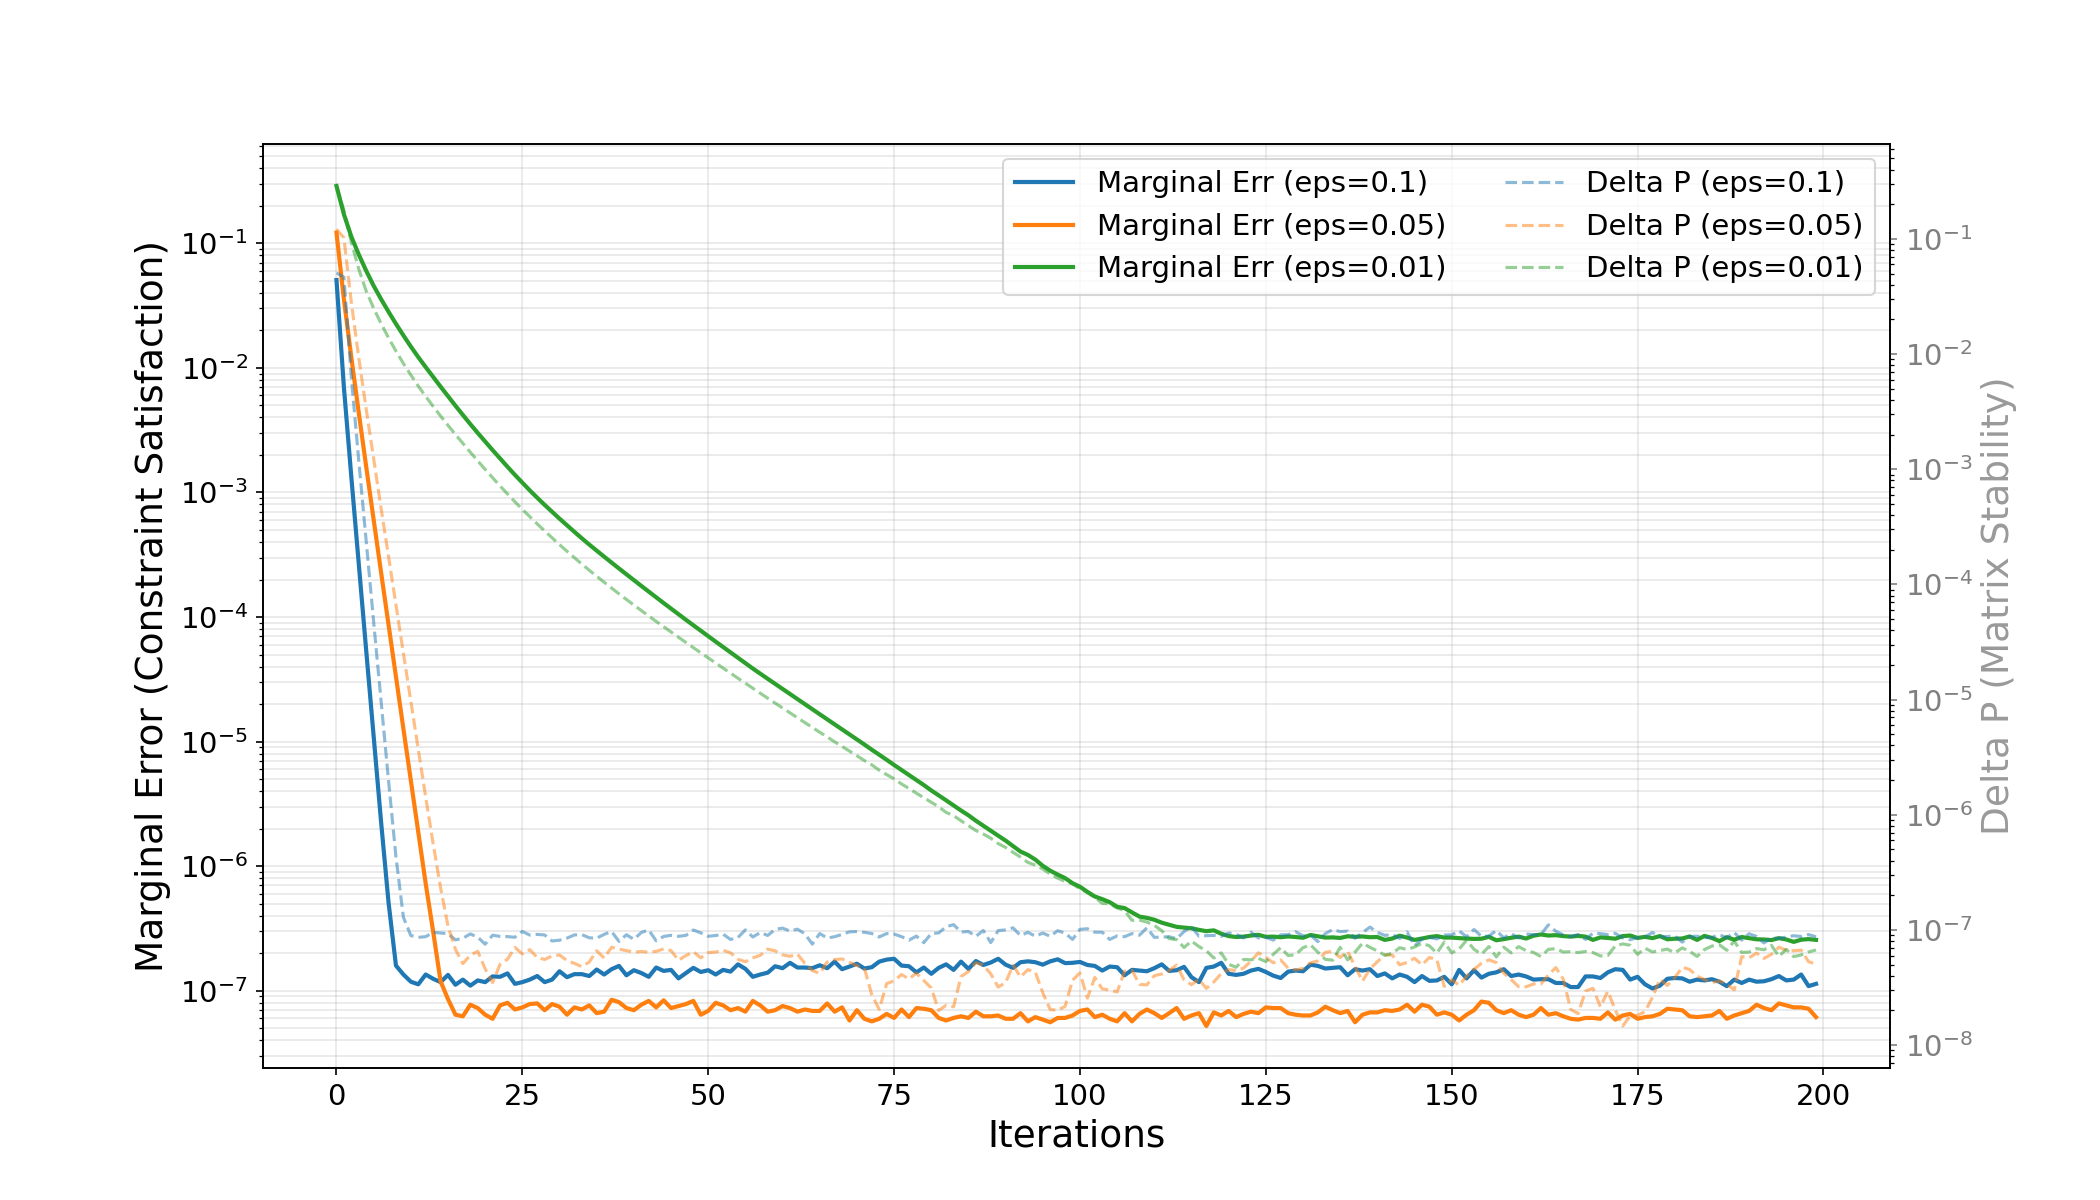
\includegraphics[width=1\linewidth]{author-kit-CVPR2026-v1-latex-/figs/sinkhorn_convergence_comparison.png}
    \caption{Sinkhorn Convergence Analysis. The plot illustrates the impact of different entropic regularization parameters ($\epsilon$) on the convergence rates of Marginal Error (representing constraint satisfaction) and Delta P (representing pointwise matrix stability). The results are obtained using a randomly initialized cost matrix $C$.}
    % The results are obtained using a randomly initialized cost matrix $C$ as a numerical stress test to verify the algorithm's robustness across arbitrary cost distributions.
    \label{fig:sensitivity_entropy}
\end{figure}

\subsection{Qualitative Results}
Qualitative results of the frame-level text-motion alignment are illustrated in \Cref{fig:qual1}. Compared to the VLM and stepwise uniform baselines, the transport matrix $\mathbf{P}$ generated by our model shows superior structural correspondence with the ground truth $\mathbf{P}^{gt}$. Notably, for captions containing action-bearing phrases that encompass extended temporal spans, our model effectively captures these long-range dependencies. For instance, in sample (a), the first three action phrases in $\mathbf{P}$ demonstrate a relatively uniform probability distribution across the corresponding frames. This highlights the effectiveness of our framework in modeling complex many-to-many alignments between motion and text, a challenging scenario where the VLM baseline falls short.